\documentclass[11pt]{article}

% Submission (anonymous double-blind) version. Switch "review" -> "final" for camera-ready.
\usepackage[review]{acl}

\usepackage[T1]{fontenc}
\usepackage[utf8]{inputenc}
\usepackage{inconsolata}
\usepackage{graphicx}
\usepackage{booktabs}
\usepackage{amsmath}
\usepackage{amssymb}
\usepackage{xcolor}
\graphicspath{{../figures/}}

\newcommand{\rcps}{\textsc{RCPS}}

\title{Retrieval-Conditional Parsing Score (RCPS):\\Choosing Document Parsers by Retrieval, Not by Appearance}

\author{Anonymous ACL submission}

\begin{document}
\maketitle

\begin{abstract}
Document parsers for retrieval-augmented generation (RAG) are commonly selected by intrinsic quality metrics---text fidelity, boundary clarity---although a production pipeline ultimately depends on whether the parsed content can be \emph{retrieved}. Building a RAG system over Korean government documents, we find the assumption fails operationally: parser selection alone moves retrieval Hit@1 by $35.2$ absolute percentage points ($0.197 \rightarrow 0.549$, a $2.8\times$ relative increase), and the parsers with the cleanest chunk boundaries rank near the bottom under retrieval. We introduce the Retrieval-Conditional Parsing Score (\rcps{}), a training-free selection protocol that ranks the parsers and chunkers a team should deploy using a held-out Q--A probe, averaging over multiple retrievers, with format-normalised answer matching; and a retriever-free coverage diagnostic that attributes missing answers to parser omission versus chunk-boundary splitting before any retriever is run. On our production pipeline $20.2\%$ of gold answers are absent from the parser output---constant across eight chunkers---while at most $2.3\%$ are split, so re-chunking cannot recover the loss; parser choice spans an \rcps{} range of $0.51$ against $0.06$ for chunker choice. Controlled cross-domain perturbations (OHR-Bench) confirm the mechanism: semantic noise collapses retrieval while boundary metrics barely move. Finally, we bound parser-side training: retrieval-aware preference optimisation lifts OHR-Bench Hit@5 by $+0.85$~pp, but a simpler fidelity-distillation control achieves $+1.22$~pp with substantially overlapping confidence intervals---we find no evidence that retrieval-reward-based selection improves over fidelity-based selection. We release KoGovDoc-RAG, a Korean document-RAG benchmark, with a reference implementation of \rcps{}.
\end{abstract}

\section{Introduction}

\begin{figure*}[t]
\centering
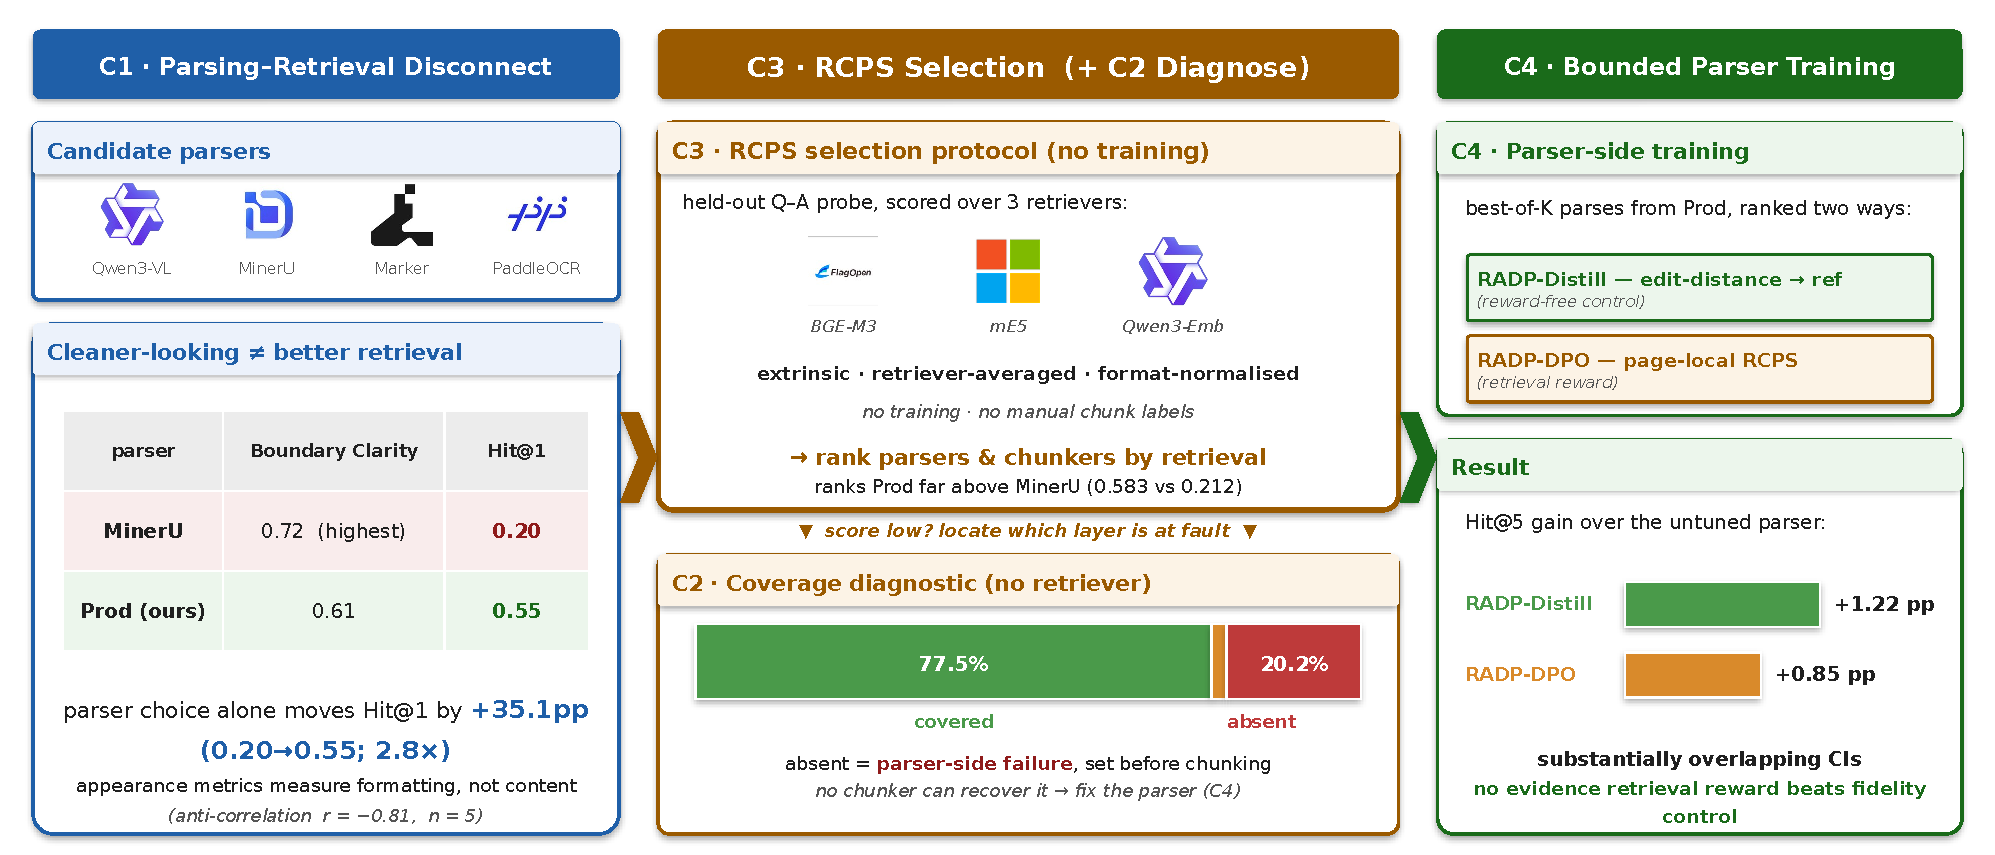
\includegraphics[width=0.8\textwidth]{fig_overview.pdf}
\caption{\textbf{Overview.} \textbf{(C1)} Selecting a document parser by appearance (Boundary Clarity) rather than retrieval is a trap: MinerU has the highest Boundary Clarity yet the lowest Hit@1, and parser choice alone moves Hit@1 by $35.2$ points ($2.8\times$; scalar correlations illustrative, \S\ref{sec:c1c2}). \textbf{(C2)} A retriever-free coverage diagnostic localises the gap to the parser---$20.2\%$ of answers are absent from the parser output, constant across all eight chunkers. \textbf{(C3)} \rcps{} selects parsers and chunkers by retrieval over a held-out Q--A probe and three retrievers, with no training. \textbf{(C4)} Parser-side training is a bounded lever: the fidelity-distillation control and the retrieval-reward variant have substantially overlapping CIs---no evidence the retrieval reward helps.}
\label{fig:overview}
\end{figure*}

Retrieval-augmented generation (RAG) is increasingly deployed over real-world document collections---government records, enterprise reports, technical manuals---that exist only as scanned or born-digital PDFs. Every such pipeline begins with a document parser that converts each page to text, which is then chunked, embedded, and retrieved. Because the parser sits at the head of the pipeline its errors cascade downstream; the practical question is how to choose it. Faced with many candidates, practitioners rank them by intrinsic parsing-quality metrics that reward clean-looking output---low text-edit distance, high boundary clarity \citep{zhao2025moc}---on the assumption that cleaner output retrieves better.

We hit this problem building a production RAG system over Korean government documents, and found the assumption fails operationally. A team ranking by intrinsic metrics would deploy MinerU \citep{mineru2025}, whose boundary-clarity score ($0.72$) is matched only by Marker; yet its retrieval Hit@1 is $0.20$, against the $0.50$--$0.55$ of three lower-scoring vision--language parsers---$35.2$ absolute Hit@1 percentage points ($2.8\times$ relative) from parser selection alone. On our parser set, Boundary Clarity ranks the candidates in nearly the opposite order from retrieval (Pearson $r = -0.81$, $n = 5$; sensitive in sign to the corpus), but the robust signal is the mechanism: on a cross-domain English check (OHR-Bench, \citealp{zhang2024ohr}), injecting semantic noise collapses retrieval while Boundary Clarity barely moves, so the intrinsic metric cannot perceive the content corruption retrieval depends on. Selection by appearance optimises a quantity structurally blind to retrievability---at least for the scanned, layout-heavy documents we study.

The question this paper answers is operational: \emph{given candidate parsers and chunkers, how should a production team pick what to deploy---and is parser training worth the cost?} Our central contribution is the \rcps{} protocol, a training-free procedure that selects the parser and chunker by what retrieval does with their output (C3). We support it with an empirical characterisation of the parsing--retrieval disconnect that motivates retrieval-grounded selection (C1), a coverage diagnostic that localises failures to the parser or chunker layer (C2), and a secondary investigation showing that parser-side training provides only bounded gains beyond selection (C4).

Figure~\ref{fig:overview} previews all four.

We release \textbf{KoGovDoc-RAG}, a Korean document-RAG benchmark of 663 question--answer pairs over 294 pages, with a reference implementation of \rcps{} and the RADP checkpoints.

\section{Related Work}

\paragraph{Diagnosing the parsing--retrieval gap.} OHR-Bench \citep{zhang2024ohr} measures the cascading impact of OCR noise on RAG; EnterpriseDocBench \citep{enterprisedocbench2026} reports a weak parsing-quality--retrieval correlation; concurrent analyses agree \citep{goodocr2026, song2026ocr}. Parsing benchmarks still rank parsers by intrinsic fidelity \citep{ouyang2025omnidocbench}---the signal C1 shows is misleading---and vision-based retrieval \citep{faysse2024colpali} sidesteps text parsing, orthogonal to the text pipelines we target. None provides a reusable selection protocol or fault localisation---which our \rcps{} (C3) and coverage diagnostic (C2) supply.

\paragraph{Training-time methods, by pipeline layer.} Retrieval-oriented training exists at every layer except the parser: chunking \citep{jina2024late, duarte2024lumber, zhao2024meta, zhao2025moc, singh2024chunkrag}, contrastive embedding \citep{conti2025insent, zhao2025lmar}, and retriever- or reader-side tuning \citep{nguyen2024rewardrag, chia2025mlongdoc, yan2025rpo}. Parsers are themselves trained---with RL on edit-distance and layout rewards \citep{infinity_parser} or query-driven for efficient RAG \citep{agenticocr}---but not on a retrieval signal; we test that signal and find it adds nothing over the fidelity reward such training already uses (C4). Our primary contributions (C1--C3) sit upstream of any training.

\section{The RCPS Protocol}

\subsection{\rcps{}: Retrieval-Conditional Parsing Score}
\label{sec:rcps}

\rcps{} ranks parsers by what downstream retrieval does with their output, not by how clean it looks. It is not a new similarity function but an evaluation protocol wrapping ordinary retrieval MRR in three choices, each removing a failure mode our experiments exhibit: (i) it is \emph{extrinsic}, scoring a held-out Q--A probe on the parsed corpus, because intrinsic text metrics reward formatting that retrieval does not depend on (\S\ref{sec:c1c2}); (ii) it is \emph{retriever-agnostic}, averaging over several embedders, because a single embedder can silently flip the top-ranked parser (Table~\ref{tab:ablation}); and (iii) it uses \emph{format-normalised exact-span relevance}, counting a chunk relevant iff it contains the answer span under shared whitespace/markdown normalisation (on our grid: $0.02$--$0.03$ score shifts, no reordering). Throughout, the \emph{\rcps{} score} is the aggregate value of Equation~\ref{eq:rcps}; the \emph{\rcps{} protocol} is the complete procedure---probe, retriever averaging, format-normalised relevance. The contribution is the protocol, not the scoring function (\S\ref{sec:c3}).

Given a parser $P$, a Q--A set $D = \{(q_i, a_i, \text{page}_i)\}$, a set of retrievers $R$, and cutoffs $K$, \rcps{} averages MRR across the cross-product:
\begin{equation}
\label{eq:rcps}
\text{RCPS}(P) = \frac{1}{|R|\,|K|} \sum_{r \in R} \sum_{k \in K} \text{MRR}@k(r, P, D).
\end{equation}
We use $R = \{$BGE-M3 \citep{chen2024bgem3}, multilingual-e5-large \citep{wang2024me5}, Qwen3-Embedding-8B \citep{qwen3emb}$\}$ and $K = \{1, 5, 10\}$. A chunk is relevant iff its source page matches the answer's and the gold span is a substring under whitespace- and markdown-insensitive normalisation. Figure~\ref{fig:protocol} sketches the protocol; the implementation is released.

\begin{figure}[t]
\centering
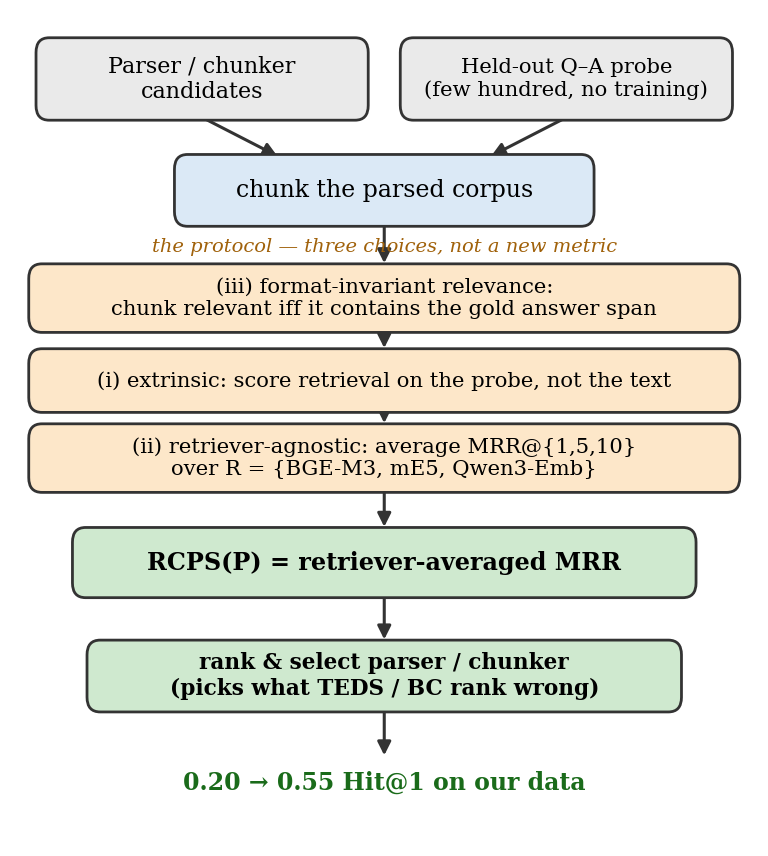
\includegraphics[width=0.66\columnwidth]{fig_rcps_protocol.png}
\caption{\rcps{} as a protocol, not a new scoring function (C3): ordinary retrieval MRR wrapped in a held-out Q--A probe, retriever-averaging, and format-normalised relevance. Run with no training, it ranks the parser and chunker a team would deploy.}
\label{fig:protocol}
\end{figure}

\paragraph{Running the protocol.} A team (1) holds out a probe of a few hundred Q--A whose answers occur verbatim in the corpus (ours are LLM-generated and judge-filtered, \S\ref{sec:setup}); (2) parses the evaluation pages once per candidate; (3) chunks, embeds with the $|R|$ retrievers, and computes Equation~\ref{eq:rcps}; (4) deploys the arg-max. \rcps{} is an offline procedure---for $m$ parsers, $c$ chunkers, and $r$ retrievers, $m$ parse runs and $m c r$ indexing-and-retrieval evaluations---with no model training and no manual chunk-level relevance annotation (relevance derives automatically from the gold span and source page). Holding the parse fixed instead ranks chunkers with the same probe. \rcps{} returns a ranking under a fixed probe, not an absolute score.

\subsection{Coverage Diagnostic --- Locating the Gap (Parser vs Chunker)}
\label{sec:coverage}

\rcps{} scores the parser, chunker, and retriever jointly, so a low score does not localise the fault. We separate the parser from the chunker with a retriever-free diagnostic: holding the parser output fixed and varying the chunker, we classify each gold answer as \emph{covered} (inside a single chunk, retrievable); \emph{split} (present in the page text but cut across chunks---a chunker-side failure, recoverable with overlap); or \emph{absent} (not found in the parser output under the same normalisation---a parser-side coverage failure: no chunker can recover content the parsed text lacks). Coverage is the ceiling on retrieval (split and absent score zero); the split/absent breakdown decides whether a parser-side fix can help (\S\ref{sec:c1c2}). Relevance reuses \rcps{}'s format-normalised matching.

\begin{figure}[t]
\centering
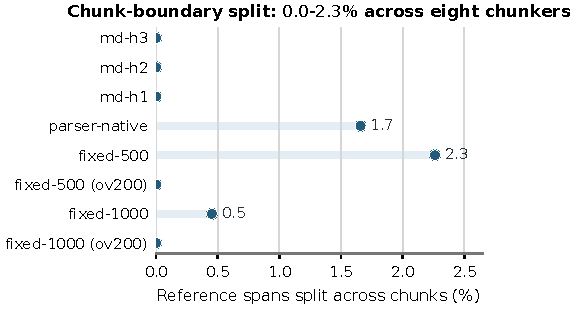
\includegraphics[width=0.78\columnwidth]{fig_coverage.pdf}
\caption{The coverage diagnostic (C2): with the parser fixed (Prod) and the chunker varied, each gold answer is \emph{covered}, \emph{split} (a chunker fault, recoverable with overlap), or \emph{absent} (a parser fault, unrecoverable by chunking). The absent rate is $\approx\!20.2\%$ and essentially constant across all eight chunkers, while split is at most $2.3\%$ (\S\ref{sec:c1c2})---chunking cannot close a gap the parser already lost.}
\label{fig:coverage}
\end{figure}

\section{Experiments}

\subsection{Setup}
\label{sec:setup}

We construct \textbf{KoGovDoc-RAG}: 663 Q--A pairs over 294 pages of Korean government documents, generated with the OpenAI \texttt{gpt-5.4-2026-03-05} model and verified by an LLM-as-judge against the teacher-distilled reference markdown (Qwen3-VL-30B pseudo-labels; 100 eval Q--A sampled, 94/100 accept). For RADP-aux's full-scale training we additionally generate 6{,}164 Q--A on the 2{,}667-page Prod training set. Cross-domain replication uses OHR-Bench \citep{zhang2024ohr} (seven domains, 2{,}264 verbatim-answerable Q--A; its Law\,$+$\,Manual subset of 1{,}043 Q--A is used only for the data-mix-sensitivity comparison in \S\ref{sec:c1c2}) across the three released parser outputs (gt, MinerU, Qwen2.5-VL) plus twelve controlled noise perturbations.

Throughout, \textbf{Prod} denotes our production parser, a Qwen3-VL-2B model \citep{qwen3vl} fine-tuned for Korean document parsing; all training deltas are measured against it. RADP-aux uses a 73-page held-out fold (202 Q--A); RADP-DPO, SimPO, and the \S\ref{sec:mechanism} analysis use the combined 242-page fold (train $\cup$ eval, 663 Q--A), with preference pairs built only from the 169-page train fold. The same 663 Q--A occupy 242 of the 294 KoGov pages; the coverage diagnostic (\S\ref{sec:c1c2}) runs over Prod's full 294-page output, the extra 52 Q--A-free pages acting as distractors. Parses for the 12-variant comparison (\S\ref{sec:c4}) use deterministic decoding (temperature 0, max 1536 tokens). We fine-tune with LoRA \citep{hu2021lora} ($r = 8$, $\alpha = 32$), sweeping $\lambda \in \{0, 0.1, 0.3, 0.5\}$ for RADP-aux ($\lambda = 0$ drops the contrastive term; the sweep is read within the aux family, Table~\ref{tab:mechanism}). \rcps{} uses the three retrievers and cutoffs of \S\ref{sec:rcps}; we report paired percentile-bootstrap 95\% CIs (1{,}000 resamples), preserving Q--A pairing across systems.

\subsection{The Parsing--Retrieval Disconnect and Coverage Diagnostic (C1--C2)}
\label{sec:c1c2}

\paragraph{Korean government documents (Figure~\ref{fig:disconnect}; full grid in Table~\ref{tab:grid}, \S\ref{sec:c3}).} \rcps{} spans $0.07$--$0.58$ across the six parsers---vision--language parsers on top, OCR systems trailing. The Qwen3-VL-30B teacher and the deployable 2B Prod form a near-tied top tier (\rcps{} $0.584$ and $0.583$), so Figure~\ref{fig:disconnect}b contrasts Prod against the appearance-ranked MinerU. The intrinsic Boundary Clarity metric \citep{zhao2025moc} anti-correlates with \rcps{} at Pearson $r = -0.81$ ($n = 5$, excluding PaddleOCR, whose BC is undefined): the two cleanest-boundary parsers (MinerU, Marker; BC $\approx 0.72$) land near the bottom, while the lower-BC vision--language parsers retrieve best (robust to dropping Marker: $n = 4$, $r = -0.74$). MoC's Chunk Stickiness is similarly disconnected ($r = +0.26$); neither intrinsic axis predicts \rcps{}.

\begin{figure*}[t]
\centering
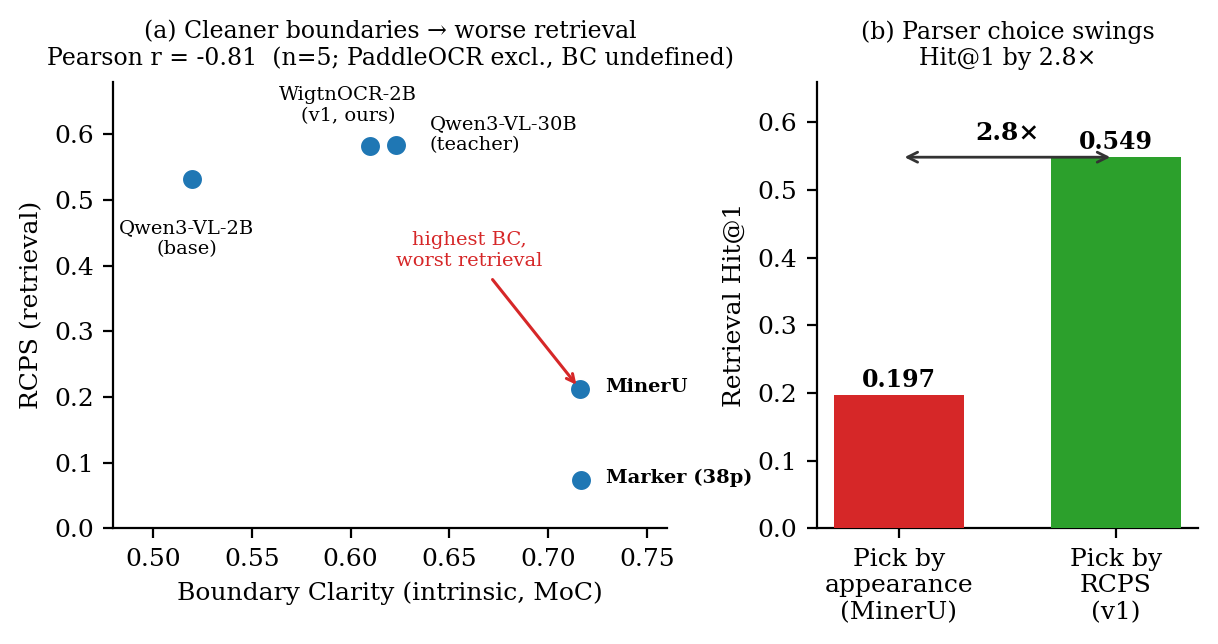
\includegraphics[width=0.72\textwidth]{fig_disconnect.png}
\caption{The parsing--retrieval disconnect on Korean government documents. (a) Boundary Clarity (intrinsic, MoC) anti-correlates with \rcps{} across parsers (Pearson $r = -0.81$, $n = 5$; PaddleOCR excluded as its BC is undefined): the cleanest-boundary parsers MinerU and Marker land near the bottom, while the lower-BC vision--language parsers retrieve best. (b) Choosing the parser by \rcps{} (Prod) rather than by appearance (MinerU) improves retrieval Hit@1 by $35.2$ absolute percentage points ($0.197 \rightarrow 0.549$; $2.8\times$ relative).}
\label{fig:disconnect}
\end{figure*}

\paragraph{Cross-domain: the mechanism.} Across all seven OHR-Bench domains (2{,}264 Q--A) we evaluate 15 parser-output variants---three released outputs plus twelve controlled noise perturbations (Appendix~\ref{app:noise}). Within each semantic-noise family, Boundary Clarity stays flat while \rcps{} collapses: for the MinerU family BC holds at $0.71$--$0.74$ from clean to severe while \rcps{} falls $-51\%$, with GOT and Qwen2.5-VL showing the same direction (Table~\ref{tab:noise}). Semantic noise that destroys retrievable content does not lower Boundary Clarity: the intrinsic metric sees formatting, not content.

The aggregate cross-variant correlation is sensitive to the document mix: Pearson BC$\leftrightarrow$\rcps{} across all 15 variants is $-0.35$ on Law\,$+$\,Manual alone but $+0.25$ on the full seven-domain corpus. We therefore report the per-family mechanism, which reproduces in every domain, as the robust finding, and treat the cross-variant scalar as illustrative only.

\paragraph{Locating the gap: parser or chunker? (Figure~\ref{fig:coverage}; per-chunker table in Appendix~\ref{app:coverage}).} The disconnect shows that intrinsic metrics mislead, but not which pipeline layer is at fault. Applying the \S\ref{sec:coverage} classification with no retriever to Prod's output (294 pages, 663 Q--A), $20.2\%$ of answers are absent and at most $2.3\%$ split, with the absent rate constant across all eight chunkers---the boundary-independence a parser fault must show. Roughly one answer in five is never produced, so no re-chunking recovers it: the gap is a parser problem, motivating the training in \S\ref{sec:c4}.

\subsection{\rcps{} Selects Both Parsers and Chunkers (C3)}
\label{sec:c3}

\begin{table}[t]
\centering\footnotesize
\setlength{\tabcolsep}{2.5pt}
\begin{tabular}{lcccc}
\toprule
Parser & BC & CS & \rcps{} & Hit@1 \\
\midrule
Qwen3-VL-30B (teacher) & 0.623 & 3.38 & \textbf{0.584} & 0.545 \\
Prod (ours, 2B) & 0.610 & 3.07 & 0.583 & 0.549 \\
Qwen3-VL-2B (base) & 0.520 & 3.74 & 0.532 & 0.500 \\
MinerU & 0.716 & 2.81 & 0.212 & 0.197 \\
PaddleOCR & --- & 3.46 & 0.140 & 0.125 \\
Marker (38p) & \textbf{0.717} & 3.41 & 0.073 & 0.068 \\
\bottomrule
\end{tabular}
\caption{The KoGov six-parser grid (\rcps{} averaged over three retrievers; Marker on its 38-page subset). Simultaneously the C1 evidence---BC anti-correlates with \rcps{}, $r = -0.81$ ($n = 5$; PaddleOCR excluded, BC undefined); CS similarly uninformative ($r = +0.26$; scale differs from Table~\ref{tab:mechanism})---and the C3 deliverable: the deployment ranking a team reads off.}
\label{tab:grid}
\end{table}

\paragraph{Selecting parsers.} A selection protocol must separate the alternatives a practitioner actually compares. The six-parser grid of \S\ref{sec:c1c2} (Table~\ref{tab:grid}, Figure~\ref{fig:disconnect}) is itself an \rcps{} ranking: it tells a team that Prod (\rcps{} $0.583$, Hit@1 $0.55$) beats MinerU ($0.21$, $0.20$) by $2.8\times$, the ordering Boundary Clarity inverts. Both appearance-ranked leaders (MinerU, Marker) sit in the grid's bottom half, and the spread \rcps{} resolves---$0.073$ to $0.584$---is the full range of deployment outcomes. Within the near-tied top tier (30B vs Prod), deployment constraints---latency, compute---decide, not retrieval.

\paragraph{Selecting chunkers.} On a fixed Prod output, the same probe separates four chunking strategies cleanly---markdown-header (md-h3, \rcps{} $0.593$) $>$ parser-native ($0.583$) $>$ LumberChunker \citep{duarte2024lumber} ($0.557$) $>$ fixed-size ($0.535$)---whereas intrinsic boundary metrics rank them inconsistently, or rank fixed-size highest because its boundaries are clean by construction. The chunker spread ($0.06$) is nearly an order of magnitude smaller than the parser spread ($0.51$), as the coverage diagnostic predicts (at most $2.3\%$ chunker-recoverable, \S\ref{sec:c1c2}): chunking moves retrieval only within the band the parser sets. One probe set thus ranks both knobs---and says which is worth turning first.

\paragraph{\rcps{} is not single-embedder MRR (Table~\ref{tab:ablation}).} The contribution of \rcps{} is not a new retrieval metric but an operational evaluation package---downstream scoring, retriever averaging, and format-normalised relevance under a shared probe (\S\ref{sec:rcps}). The single-embedder ablation is a secondary illustration of retriever sensitivity: the overall rankings remain similar (Kendall $\tau = 0.87$), but BGE-M3 alone reverses the near-tied top pair ($0.583$ vs $0.584$)---a flip a team trusting its production embedder inherits silently. Format-normalised matching shifts every score by $0.02$--$0.03$ without reordering.

\begin{table}[t]
\centering\footnotesize
\setlength{\tabcolsep}{3pt}
\begin{tabular}{lcc}
\toprule
Protocol configuration & Top pair & $\tau$ vs \rcps{} \\
\midrule
naive MRR (1 embedder) & Prod $\succ$ 30B & 0.87 \\
$+$ retriever-averaging & 30B $\succ$ Prod & 1.00 \\
$+$ format-normalised & Prod $\succ$ 30B & 0.87 \\
full \rcps{} & 30B $\succ$ Prod & --- \\
\bottomrule
\end{tabular}
\caption{\rcps{} protocol ablation on the KoGov six-parser grid: only the inverted top pair is shown; the lower ranks (Qwen3-VL-2B $\succ$ MinerU $\succ$ PaddleOCR $\succ$ Marker) are identical throughout. Retriever-averaging alone flips the top pair. Kendall $\tau$ is over the full ranking; ``30B'' $=$ the Qwen3-VL-30B teacher.}
\label{tab:ablation}
\end{table}

\subsection{Parser-Side Training Is a Bounded, Reward-Agnostic Lever (C4)}
\label{sec:c4}\label{sec:mechanism}

Having identified parser-side content loss as the dominant bottleneck (\S\ref{sec:c1c2}), we ask whether parser training adds anything beyond selection. We evaluate two retrieval-aware parser interventions (Retrieval-Aware Document Parsing, RADP)---a hidden-state auxiliary loss (RADP-aux) and discrete-output DPO on a page-local \rcps{} reward (RADP-DPO) \citep{rafailov2023dpo}---against RADP-Distill, a matched control selecting candidates by edit distance to the reference markdown with no retrieval reward, plus reference-free SimPO \citep{meng2024simpo} as a further preference-optimisation control. Among the retrieval-aware variants, only RADP-DPO yields a statistically significant positive gain on the confirmatory OHR-Bench evaluation---the auxiliary loss is sub-threshold and SimPO negative---at $+0.85$~pp Hit@5 $[+0.35, +1.43]$ (KoGov $\approx{+}2$~pp, exploratory); R2 is our primary retrieval-aware variant (clearest cross-domain fidelity improvement), with the reward-sharpened R3 reported for completeness. RADP-Distill achieves $+1.22$~pp $[+0.35, +2.15]$ (Table~\ref{tab:c4}); the effect-size intervals overlap substantially, and \textbf{we find no evidence that retrieval-reward-based candidate selection improves over fidelity-based candidate selection} at the confirmatory endpoint---the lever is text fidelity, not chunking. Recipe, per-variant results, full metric grid (Table~\ref{tab:ohr}), and mechanism statistics: Appendices~\ref{app:milestones}--\ref{app:mechanism}.

\begin{table}[t]
\centering\scriptsize
\setlength{\tabcolsep}{2.5pt}
\begin{tabular}{llc}
\toprule
Variant & Selection signal & $\Delta$Hit@5 [95\% CI] \\
\midrule
RADP-Distill & ref.\ edit dist. & $\mathbf{+1.22}$ $[{+}0.35, {+}2.15]$ \\
RADP-DPO-R2 & page-local \rcps{} & $+0.85$ $[{+}0.35, {+}1.43]$ \\
RADP-DPO-R3 & $+$ hard negatives & $+1.03$ $[{+}0.24, {+}1.84]$ \\
\bottomrule
\end{tabular}
\caption{C4 at the confirmatory endpoint: OHR-Bench $\Delta$Hit@5 vs Prod, pp (2{,}264 Q--A, seven domains, three-retriever macro, paired bootstrap). Fidelity control and retrieval-reward variants have substantially overlapping intervals---no evidence the reward improves over the control. RADP-aux is sub-threshold, SimPO negative (Appendix~\ref{app:dpo}).}
\label{tab:c4}
\end{table}

\section{Discussion and Conclusion}

\paragraph{Selection, not training, is the headline.} The largest effect is not a training method: selecting the parser by retrieval (\rcps{}) instead of intrinsic metrics moves Hit@1 by $35.2$ points ($2.8\times$, \S\ref{sec:c1c2}). Parser-side training is a bounded, secondary lever ($\approx$1~pp Hit@5), with no evidence the retrieval reward beats fidelity distillation (\S\ref{sec:c4}).

\paragraph{Why the diagnosis and the mechanism agree.} ``Clean'' splits into two axes: Boundary Clarity measures formatting, TextNED content. MinerU is formatting-clean but loses content (C1); training improves fidelity with the formatting signature unchanged (TextNED $0.240 \rightarrow 0.158$, BC $0.630 \rightarrow 0.641$; Table~\ref{tab:mechanism}, \S\ref{sec:mechanism}).

\paragraph{Playbook and conclusion.} For practitioners: (1) select parsers with \rcps{} (a few hundred Q--A, no training); (2) run the coverage diagnostic---fix the chunker if \emph{split}, the parser if \emph{absent}; (3) if you train, distil toward clean reference text---retrieval-aware methods must first beat that control; (4) gains concentrate on factoid queries (layout-heavy mixes: tune the chunker/embedder).

\section*{Limitations}

\paragraph{Single primary language and statistical power.} The C1 diagnostic is strongest in Korean ($n = 5$, $r = -0.81$). On English OHR-Bench the aggregate cross-variant scalar is sign-sensitive to document mix ($r = -0.35$ on Law\,$+$\,Manual, $+0.25$ on the full seven-domain corpus), so directional consistency holds only for the per-family noise mechanism (\S\ref{sec:c1c2}), which replicates in every domain---not for the scalar correlation. The English evidence is also built on three real parser outputs plus twelve controlled perturbations rather than fifteen independent parsers. With these sample sizes the correlations are illustrative rather than inferential.

\paragraph{Q--A generation and construct validity.} The KoGov reference markdown is itself pseudo-ground-truth distilled from a Qwen3-VL-30B teacher (with manual de-noising of contaminated samples), and the Q--A were LLM-generated and checked by an LLM-as-judge against that reference (94/100 accept on a 100-Q--A stratified sample); neither the reference parses nor the queries were fully human-verified. Synthetic queries and pseudo-reference bound what \rcps{} can claim absolutely, but the exposure is narrow: our comparative findings---the $2.8\times$ parser-choice swing and every parser/chunker ranking---hold the Q--A set fixed across systems and so are internally valid regardless of how queries were generated, and the confirmatory cross-domain test (\S\ref{sec:c4}) uses OHR-Bench's own externally curated Q--A. We release the frozen KoGov eval set for audit.

\paragraph{KoGov is exploratory; OHR-Bench is confirmatory.} The headline KoGov cell (R2 $+1.96$~pp, Table~\ref{tab:kogov}) has a paired 95\% interval of $[-1.06, +5.03]$---two-sided non-significant and selected from a multi-cell scan---so we claim no two-sided significance on KoGov. The confirmatory evidence is the pre-specified OHR-Bench replication (R2 $+0.85$~pp $[+0.35, +1.43]$, $n = 2{,}264$). A larger KoGov fold ($\ge 1{,}500$ Q--A) would be needed for a powered two-sided result.

\paragraph{Candidate pool and untested paradigms.} Preference pairs are sampled from Prod itself; an alternative pool (e.g.\ chosen/rejected pairs from other parsers) might shift the mechanism away from reference-fidelity, which we did not test. We also test only the hidden-state auxiliary loss, discrete-output DPO with a reference policy, and reference-free SimPO; token-level RL, multi-task interleaving, curriculum schedules, and chunk-granularity oracle distillation are untested. Finally, RADP-DPO is a parser-layer intervention; chunker-, embedder-, and reranker-side training on \rcps{}-graded chunks are complementary directions left to future work.

\bibliography{refs}

\appendix

\section{RADP-DPO Milestone Construction}
\label{app:milestones}

This appendix details RADP-DPO, the discrete-output retrieval-aware intervention of \S\ref{sec:c4}: it samples multiple parses from the production parser Prod (Qwen3-VL-2B fine-tuned for Korean document parsing), ranks them by page-local \rcps{} score (Equation~\ref{eq:rcps} restricted to the page's questions), and converts candidate pairs with a sufficient reward gap into DPO preferences. Pages come from the 169-page KoGov train fold.

For each train page we sample $K$ alternative parses from the production parser, chunk and score each by a page-local \rcps{} (the page's questions against the parse's own chunks plus distractors), and form preference pairs (chosen $=$ higher-\rcps{} parse, gap $\ge 5$~pp). The reward is sharpened across three milestones: \textbf{R1} ($K = 2$ parses, uniform distractors, $\beta = 0.1$) $\rightarrow$ \textbf{R2} (a warm-started iterative round, $\beta = 0.05$) $\rightarrow$ \textbf{R3} ($K = 14$ parses with a full-corpus hard-negative pool---the other-page chunks closest to the page's queries---widening the candidate-score gap from about $0.05$ to $0.56$). We train with a LoRA-toggle reference ($\pi_\theta =$ LoRA on, $\pi_\text{ref} =$ LoRA off):
\begin{equation}
\mathcal{L}_\text{DPO} = -\log \sigma\big(\beta\,[\Delta_\theta - \Delta_\text{ref}]\big),
\end{equation}
where $\Delta_\bullet = \log \pi_\bullet(c) - \log \pi_\bullet(r)$ for the chosen ($c$) and rejected ($r$) parse.
The reference-free SimPO control ($\beta = 2.0$, $\gamma = 1.0$) removes the reference policy entirely.

\section{KoGov DPO Progression, RADP-aux Sweep, SimPO, and Robustness}
\label{app:dpo}

This appendix reports the complete parser-training results underlying \S\ref{sec:c4}: the RADP-DPO milestone progression (R1--R3, constructed in Appendix~\ref{app:milestones}), the RADP-aux sweep, the SimPO control, and the cross-domain OHR-Bench evaluation. All systems are LoRA fine-tunes of the same production parser Prod (Qwen3-VL-2B); KoGov results use the 242-page / 663-Q--A fold against the same Prod baseline, with Hit@$k$ macro-averaged over the three retrievers BGE-M3, multilingual-e5-large, and Qwen3-Embedding-8B; Table~\ref{tab:ohr} and the robustness paragraph concern OHR-Bench (2{,}264 English Q--A, seven domains).

On the KoGov fold (10{,}000-resample paired bootstrap), the three RADP-DPO milestones improve Hit@5 on parser-native chunking over Prod along the reward-sharpening axis ($+1.96$ to $+2.11$~pp, all $P[\Delta{>}0] \approx 0.90$; per-milestone point estimates and CIs in Table~\ref{tab:kogov}). At $n = 663$ every two-sided interval spans zero, so these are exploratory: the Hit@5 / parser-native cell was selected from a multi-cell scan over (chunker $\times$ retriever $\times$ $k$) with no family-wise correction. The reward-agnostic RADP-Distill control, evaluated on the same fold, reaches $+2.61$~pp and is the headline; its powered confirmation is the pre-specified OHR-Bench replication ($+1.22$~pp Hit@5, Table~\ref{tab:ohr}).

\begin{table*}[t]
\centering\small
\setlength{\tabcolsep}{4pt}
\begin{tabular}{lccccc}
\toprule
$\Delta$ vs Prod (pp) & Hit@1 & Hit@5 & Hit@10 & MRR@10 & nDCG@5 \\
\midrule
RADP-Distill & \textbf{+0.88} & \textbf{+1.22} & \textbf{+1.32} & \textbf{+1.01} & \textbf{+1.05} \\
RADP-DPO-R2 & +0.53 & +0.85 & +0.81 & +0.70 & +0.74 \\
RADP-DPO-R3 & +1.31 & +1.03 & +0.81 & +1.17 & +1.15 \\
\bottomrule
\end{tabular}
\caption{OHR-Bench cross-domain $\Delta$ vs Prod, in pp (2{,}264 Q--A over seven English domains; three-retriever macro; 1{,}000-resample paired bootstrap). The Hit@5 deltas are two-sided significant (95\% CIs: RADP-Distill $[+0.35, +2.15]$, R2 $[+0.35, +1.43]$, R3 $[+0.24, +1.84]$). The other columns are monotone re-cuts of the same per-system ranked list, reported only because practitioners use different cutoffs. RADP-Distill leads at the primary metric Hit@5; R3 reaches higher Hit@1 and MRR@10 point estimates but with overlapping CIs---no evidence the retrieval reward helps at the powered endpoint (\S\ref{sec:c4}).}
\label{tab:ohr}
\end{table*}

\begin{table*}[t]
\centering\small
\setlength{\tabcolsep}{3pt}
\begin{tabular}{lcccc}
\toprule
Variant (vs Prod $=0.6863$) & Hit@5 & $\Delta$Hit@5 [95\% CI] & $P[\Delta{>}0]$ & $\Delta$\rcps{} \\
\midrule
RADP-DPO-R3 & 0.7074 & $+2.11$ $[{-}0.96, {+}5.13]$ & 0.913 & $+1.72$ \\
RADP-DPO-R1 & 0.7069 & $+2.06$ $[{-}0.96, {+}5.13]$ & 0.907 & $+0.57$ \\
RADP-DPO-R2 & 0.7059 & $+1.96$ $[{-}1.06, {+}5.03]$ & 0.897 & $+0.47$ \\
RADP-SimPO (ctrl) & 0.6793 & $-0.70$ $[{-}3.77, {+}2.31]$ & 0.321 & $-1.56$ \\
\bottomrule
\end{tabular}
\caption{RADP-DPO milestone progression and the SimPO control on parser-native chunking, 242-page / 663-Q--A fold, 10k paired percentile bootstrap, all against the same Prod baseline (Hit@5 $= 0.6863$). Macro Hit@$k$ averages the three retrievers of \S\ref{sec:rcps}. All three milestones are strong directional positives ($P[\Delta{>}0] \ge 0.90$) but two-sided non-significant at this fold size; RADP-SimPO is uniformly negative. The RADP-Distill headline (KoGov $\Delta$Hit@5 $+2.61$~pp) is in \S\ref{sec:c4} and Table~\ref{tab:ohr}. Across three Prod seeds the standard deviation of the mean $\Delta$Hit@5 is 0.90~pp.}
\label{tab:kogov}
\end{table*}

\paragraph{RADP-aux is sub-threshold.} The auxiliary loss peaks at $\lambda = 0.1$ ($+1$--$2$~pp \rcps{}) then declines monotonically as the contrastive objective competes with $\mathcal{L}_\text{parse}$ over the same LoRA parameters; every $\Delta$-versus-control interval includes zero and the one-sided $P[\Delta{>}0]$ never approaches 0.90. The hidden-state route does not reach the deployed markdown---only the discrete output does.

\paragraph{SimPO is negative.} The reference-free length-normalised variant gives uniformly negative deltas ($-0.7$ to $-1.7$~pp Hit@5), indicating the DPO reference policy is load-bearing: without it the parser drifts from the production distribution before any preference signal can compound.

\paragraph{Robustness.} The headline RADP-Distill OHR-Bench gain survives two checks. Because it ranks candidates by edit-distance and uses no retriever, it cannot overfit any embedder; its Hit@5 gain is near-uniform across the three (BGE-M3 $+1.06$, ml-e5-large $+1.10$, Qwen3-Emb $+1.50$~pp). And it concentrates on text-evidence (factoid) queries ($+1.19$~pp) while near-neutral on table-evidence ones ($+0.32$~pp), consistent with the text-fidelity mechanism.

\section{Chunk-Level Mechanism Statistics}
\label{app:mechanism}

This appendix examines whether the retrieval gains of \S\ref{sec:c4} arise from changes in chunk structure (boundaries, cohesion) or from improvements in parsed-text fidelity. We measure four chunk-level statistics on the 242-page KoGov fold for every trained system and Prod, the shared baseline, in Table~\ref{tab:mechanism}: MoC Boundary Clarity (BC, adjacent-chunk discontinuity), MoC Chunk Stickiness (CS, within-chunk cohesion), normalised edit distance to the reference markdown (TextNED, character-level Levenshtein distance $\div$ longer-string length), and chunking shape.

\begin{table*}[t]
\centering\small
\setlength{\tabcolsep}{3.5pt}
\begin{tabular}{lcccccc}
\toprule
Variant & len & c/pg & clen & BC$\uparrow$ & CS$\downarrow$ & TextNED$\downarrow$ \\
\midrule
Prod (ref) & 1385 & 4.82 & 274 & 0.630 & 0.474 & 0.240 \\
RADP-Distill & 1597 & 5.29 & 291 & 0.641 & --- & \textbf{0.158} \\
aux $\lambda{=}0.0$ & 799 & 2.96 & 245 & 0.553 & 0.473 & 0.626 \\
aux $\lambda{=}0.1$ & 1380 & 4.05 & 321 & 0.652 & 0.484 & 0.423 \\
aux $\lambda{=}0.3$ & 1930 & 6.73 & 272 & 0.470 & 0.475 & 0.332 \\
aux $\lambda{=}0.5$ & 2035 & 5.82 & 327 & 0.556 & 0.470 & 0.318 \\
DPO-R1 & 1606 & 4.97 & 311 & 0.646 & 0.474 & \textbf{0.167} \\
DPO-R2 & 1610 & 4.83 & 321 & 0.647 & 0.476 & \textbf{0.163} \\
DPO-R3 & 1514 & 4.88 & 300 & 0.656 & 0.485 & 0.185 \\
SimPO & 1703 & 5.31 & 305 & 0.601 & 0.470 & 0.186 \\
\bottomrule
\end{tabular}
\caption{Chunk-level mechanism statistics on the 242-page fold (len $=$ parse length, c/pg $=$ chunks per page, clen $=$ chunk length). RADP-Distill attains the lowest TextNED of all ($0.158 <$ R2's $0.163 <$ Prod's $0.240$) with BC unchanged ($0.641$, within Prod's range), confirming that text fidelity, not chunk structure, is the operative axis (CS was not measured for RADP-Distill, which uses a fixed chunking scheme). Among retrieval-reward variants, R2 has the lowest TextNED ($0.163$); R3's KoGov TextNED ($0.185$) does not beat it.}
\label{tab:mechanism}
\end{table*}

\paragraph{The signal.} All three RADP-DPO milestones reduce TextNED from Prod's $0.240$ to $0.163$--$0.185$, a 23--32\% move toward the reference markdown; R1 and R2 achieve the largest reductions ($0.167$, $0.163$). RADP-aux instead increases TextNED ($0.318$--$0.626$) because its hidden-state objective degrades surface text. TextNED is positively associated with Hit@5 (R3 the one DPO-cluster exception), and RADP-Distill reduces it furthest ($0.158$) while leading on retrieval---the cleanest demonstration that text fidelity, not the retrieval reward, is the lever.

\paragraph{Cross-domain replication.} On all 4{,}040 English OHR-Bench pages, zero-shot Prod reaches TextNED $0.192$---below its $0.240$ on Korean, so English leaves less fidelity headroom. R2 reduces it to $0.1894$ (a $-0.0026$ delta, $-1.36\%$, 95\% CI $[-0.0043, -0.0010]$, two-sided significant). R3 pushes the English value marginally lower ($0.184$) yet does not improve KoGov fidelity, which is why R2 is the headline variant.

\paragraph{The non-signal.} The MoC chunking signature is unchanged: BC for every DPO variant lands in $0.60$--$0.66$ (Prod $0.63$) and CS near $0.47$--$0.49$ (Prod $0.474$); chunks-per-page ($\sim$5) and chunk length ($300$--$321$) stay close to Prod's. The gain comes from what is parsed, not how chunks are split.

\paragraph{Secondary patterns.} The gain concentrates on text-evidence (factoid) queries ($+1.19$~pp)---where the verbatim answer span must land inside a chunk---and is near-neutral on table-evidence ones ($+0.32$~pp). Because RADP-Distill ranks by edit-distance and uses no retriever, its gain is near-uniform across the three embedders, confirming a parser-level effect rather than an embedder artefact. RADP-aux stays sub-threshold because its hidden-state signal reaches the deployed markdown only through diffuse $\mathcal{L}_\text{parse}$ back-flow, never localising to the surface tokens the retriever rewards.

\section{Coverage Diagnostic per Chunker}
\label{app:coverage}

This appendix tabulates the retriever-free coverage diagnostic of \S\ref{sec:coverage} applied to the production parser Prod (Qwen3-VL-2B) on KoGovDoc-RAG (294 pages, 663 Q--A): each gold answer is \emph{covered} (inside one chunk), \emph{split} (in the page text but cut across chunks), or \emph{absent} (not in the parser output), classified by text matching only (Table~\ref{tab:coverage}).

\begin{table}[h]
\centering\small
\begin{tabular}{lccc}
\toprule
Chunker & covered & split & absent \\
\midrule
md\_h3 & 79.8\% & 0.0\% & 20.2\% \\
parser\_native & 78.1\% & 1.7\% & 20.2\% \\
fixed500 & 77.5\% & 2.3\% & 20.2\% \\
fixed500\_ov200 & 79.8\% & 0.0\% & 20.2\% \\
\bottomrule
\end{tabular}
\caption{Answer-coverage diagnostic on Prod's output (294 pages, 663 KoGov Q--A; text matching only, no retriever). The absent rate (a parser fault) is constant at 20.2\% across all eight chunkers (four representative rows shown), the required boundary-independence check; the split rate (a chunker fault) is at most 2.3\% and vanishes under overlap. Chunkers: md\_h$\{$1,2,3$\}$ $=$ markdown-header splitting at heading depth $k$; parser\_native $=$ the parser's own segmentation; fixed~$N$[\_ov$M$] $=$ fixed $N$-character windows, optionally with $M$-character overlap.}
\label{tab:coverage}
\end{table}

\section{OHR-Bench Noise-Family Grid}
\label{app:noise}

This appendix tabulates the controlled-noise grid behind the cross-domain mechanism finding of \S\ref{sec:c1c2}: twelve OHR-Bench parser-output perturbations (three parser families $\times$ four semantic-noise severities), each scored for Boundary Clarity and \rcps{} over all seven domains (2{,}264 Q--A, three-retriever average).

\begin{table}[h]
\centering\scriptsize
\setlength{\tabcolsep}{1pt}
\begin{tabular}{lcc}
\toprule
Family & BC (clean$\to$sev.) & \rcps{} (clean$\to$sev.) \\
\midrule
MinerU & 0.735/0.708/0.715/0.712 & 0.496/0.413/0.351/0.243 \\
Qwen2.5-VL & 0.619/0.614/0.616/0.610 & 0.467/0.462/0.460/0.429 \\
GOT & --/0.634/0.495/0.650 & --/0.383/0.338/0.257 \\
\bottomrule
\end{tabular}
\caption{Per-family Boundary Clarity and \rcps{} across semantic-noise severity (clean/mild/moderate/severe) on the seven OHR-Bench domains---the source for the \S\ref{sec:c1c2} noise numbers. Within each family BC stays roughly flat while \rcps{} falls (MinerU $-51\%$). GOT has no clean baseline; the GT output and three formatting-noise variants enter only the aggregate scalar (\S\ref{sec:c1c2}) and are in the released grid.}
\label{tab:noise}
\end{table}

\end{document}
